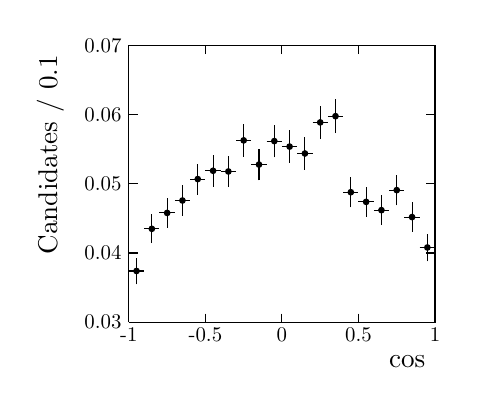
\begin{tikzpicture}
\pgfdeclareplotmark{cross} {
\pgfpathmoveto{\pgfpoint{-0.3\pgfplotmarksize}{\pgfplotmarksize}}
\pgfpathlineto{\pgfpoint{+0.3\pgfplotmarksize}{\pgfplotmarksize}}
\pgfpathlineto{\pgfpoint{+0.3\pgfplotmarksize}{0.3\pgfplotmarksize}}
\pgfpathlineto{\pgfpoint{+1\pgfplotmarksize}{0.3\pgfplotmarksize}}
\pgfpathlineto{\pgfpoint{+1\pgfplotmarksize}{-0.3\pgfplotmarksize}}
\pgfpathlineto{\pgfpoint{+0.3\pgfplotmarksize}{-0.3\pgfplotmarksize}}
\pgfpathlineto{\pgfpoint{+0.3\pgfplotmarksize}{-1.\pgfplotmarksize}}
\pgfpathlineto{\pgfpoint{-0.3\pgfplotmarksize}{-1.\pgfplotmarksize}}
\pgfpathlineto{\pgfpoint{-0.3\pgfplotmarksize}{-0.3\pgfplotmarksize}}
\pgfpathlineto{\pgfpoint{-1.\pgfplotmarksize}{-0.3\pgfplotmarksize}}
\pgfpathlineto{\pgfpoint{-1.\pgfplotmarksize}{0.3\pgfplotmarksize}}
\pgfpathlineto{\pgfpoint{-0.3\pgfplotmarksize}{0.3\pgfplotmarksize}}
\pgfpathclose
\pgfusepathqstroke
}
\pgfdeclareplotmark{cross*} {
\pgfpathmoveto{\pgfpoint{-0.3\pgfplotmarksize}{\pgfplotmarksize}}
\pgfpathlineto{\pgfpoint{+0.3\pgfplotmarksize}{\pgfplotmarksize}}
\pgfpathlineto{\pgfpoint{+0.3\pgfplotmarksize}{0.3\pgfplotmarksize}}
\pgfpathlineto{\pgfpoint{+1\pgfplotmarksize}{0.3\pgfplotmarksize}}
\pgfpathlineto{\pgfpoint{+1\pgfplotmarksize}{-0.3\pgfplotmarksize}}
\pgfpathlineto{\pgfpoint{+0.3\pgfplotmarksize}{-0.3\pgfplotmarksize}}
\pgfpathlineto{\pgfpoint{+0.3\pgfplotmarksize}{-1.\pgfplotmarksize}}
\pgfpathlineto{\pgfpoint{-0.3\pgfplotmarksize}{-1.\pgfplotmarksize}}
\pgfpathlineto{\pgfpoint{-0.3\pgfplotmarksize}{-0.3\pgfplotmarksize}}
\pgfpathlineto{\pgfpoint{-1.\pgfplotmarksize}{-0.3\pgfplotmarksize}}
\pgfpathlineto{\pgfpoint{-1.\pgfplotmarksize}{0.3\pgfplotmarksize}}
\pgfpathlineto{\pgfpoint{-0.3\pgfplotmarksize}{0.3\pgfplotmarksize}}
\pgfpathclose
\pgfusepathqfillstroke
}
\pgfdeclareplotmark{newstar} {
\pgfpathmoveto{\pgfqpoint{0pt}{\pgfplotmarksize}}
\pgfpathlineto{\pgfqpointpolar{44}{0.5\pgfplotmarksize}}
\pgfpathlineto{\pgfqpointpolar{18}{\pgfplotmarksize}}
\pgfpathlineto{\pgfqpointpolar{-20}{0.5\pgfplotmarksize}}
\pgfpathlineto{\pgfqpointpolar{-54}{\pgfplotmarksize}}
\pgfpathlineto{\pgfqpointpolar{-90}{0.5\pgfplotmarksize}}
\pgfpathlineto{\pgfqpointpolar{234}{\pgfplotmarksize}}
\pgfpathlineto{\pgfqpointpolar{198}{0.5\pgfplotmarksize}}
\pgfpathlineto{\pgfqpointpolar{162}{\pgfplotmarksize}}
\pgfpathlineto{\pgfqpointpolar{134}{0.5\pgfplotmarksize}}
\pgfpathclose
\pgfusepathqstroke
}
\pgfdeclareplotmark{newstar*} {
\pgfpathmoveto{\pgfqpoint{0pt}{\pgfplotmarksize}}
\pgfpathlineto{\pgfqpointpolar{44}{0.5\pgfplotmarksize}}
\pgfpathlineto{\pgfqpointpolar{18}{\pgfplotmarksize}}
\pgfpathlineto{\pgfqpointpolar{-20}{0.5\pgfplotmarksize}}
\pgfpathlineto{\pgfqpointpolar{-54}{\pgfplotmarksize}}
\pgfpathlineto{\pgfqpointpolar{-90}{0.5\pgfplotmarksize}}
\pgfpathlineto{\pgfqpointpolar{234}{\pgfplotmarksize}}
\pgfpathlineto{\pgfqpointpolar{198}{0.5\pgfplotmarksize}}
\pgfpathlineto{\pgfqpointpolar{162}{\pgfplotmarksize}}
\pgfpathlineto{\pgfqpointpolar{134}{0.5\pgfplotmarksize}}
\pgfpathclose
\pgfusepathqfillstroke
}
\definecolor{c}{rgb}{1,1,1};
\draw [color=c, fill=c] (0.1,4.72095) rectangle (4.9,9.16419);
\draw [color=c, fill=c] (0.772,5.43186) rectangle (4.66,8.94203);
\definecolor{c}{rgb}{0,0,0};
\draw [c] (0.772,5.43186) -- (0.772,8.94203) -- (4.66,8.94203) -- (4.66,5.43186) -- (0.772,5.43186);
\draw [c,line width=0.4] (0.8692,5.91154) -- (0.8692,6.08124);
\draw [c,line width=0.4] (0.8692,6.08124) -- (0.8692,6.25095);
\draw [c,line width=0.4] (0.772,6.08124) -- (0.8692,6.08124);
\draw [c,line width=0.4] (0.8692,6.08124) -- (0.9664,6.08124);
\foreach \P in {(0.8692,6.08124)}{\draw[mark options={color=c,fill=c},mark size=1.201201pt,mark=*,mark size=1pt] plot coordinates {\P};}
\draw [c,line width=0.4] (1.0636,6.43352) -- (1.0636,6.61654);
\draw [c,line width=0.4] (1.0636,6.61654) -- (1.0636,6.79957);
\draw [c,line width=0.4] (0.9664,6.61654) -- (1.0636,6.61654);
\draw [c,line width=0.4] (1.0636,6.61654) -- (1.1608,6.61654);
\foreach \P in {(1.0636,6.61654)}{\draw[mark options={color=c,fill=c},mark size=1.201201pt,mark=*,mark size=1pt] plot coordinates {\P};}
\draw [c,line width=0.4] (1.258,6.63058) -- (1.258,6.81838);
\draw [c,line width=0.4] (1.258,6.81838) -- (1.258,7.00618);
\draw [c,line width=0.4] (1.1608,6.81838) -- (1.258,6.81838);
\draw [c,line width=0.4] (1.258,6.81838) -- (1.3552,6.81838);
\foreach \P in {(1.258,6.81838)}{\draw[mark options={color=c,fill=c},mark size=1.201201pt,mark=*,mark size=1pt] plot coordinates {\P};}
\draw [c,line width=0.4] (1.4524,6.78488) -- (1.4524,6.97634);
\draw [c,line width=0.4] (1.4524,6.97634) -- (1.4524,7.16779);
\draw [c,line width=0.4] (1.3552,6.97634) -- (1.4524,6.97634);
\draw [c,line width=0.4] (1.4524,6.97634) -- (1.5496,6.97634);
\foreach \P in {(1.4524,6.97634)}{\draw[mark options={color=c,fill=c},mark size=1.201201pt,mark=*,mark size=1pt] plot coordinates {\P};}
\draw [c,line width=0.4] (1.6468,7.05078) -- (1.6468,7.24837);
\draw [c,line width=0.4] (1.6468,7.24837) -- (1.6468,7.44597);
\draw [c,line width=0.4] (1.5496,7.24837) -- (1.6468,7.24837);
\draw [c,line width=0.4] (1.6468,7.24837) -- (1.744,7.24837);
\foreach \P in {(1.6468,7.24837)}{\draw[mark options={color=c,fill=c},mark size=1.201201pt,mark=*,mark size=1pt] plot coordinates {\P};}
\draw [c,line width=0.4] (1.8412,7.15376) -- (1.8412,7.35368);
\draw [c,line width=0.4] (1.8412,7.35368) -- (1.8412,7.5536);
\draw [c,line width=0.4] (1.744,7.35368) -- (1.8412,7.35368);
\draw [c,line width=0.4] (1.8412,7.35368) -- (1.9384,7.35368);
\foreach \P in {(1.8412,7.35368)}{\draw[mark options={color=c,fill=c},mark size=1.201201pt,mark=*,mark size=1pt] plot coordinates {\P};}
\draw [c,line width=0.4] (2.0356,7.14518) -- (2.0356,7.3449);
\draw [c,line width=0.4] (2.0356,7.3449) -- (2.0356,7.54463);
\draw [c,line width=0.4] (1.9384,7.3449) -- (2.0356,7.3449);
\draw [c,line width=0.4] (2.0356,7.3449) -- (2.1328,7.3449);
\foreach \P in {(2.0356,7.3449)}{\draw[mark options={color=c,fill=c},mark size=1.201201pt,mark=*,mark size=1pt] plot coordinates {\P};}
\draw [c,line width=0.4] (2.23,7.53158) -- (2.23,7.7398);
\draw [c,line width=0.4] (2.23,7.7398) -- (2.23,7.94802);
\draw [c,line width=0.4] (2.1328,7.7398) -- (2.23,7.7398);
\draw [c,line width=0.4] (2.23,7.7398) -- (2.3272,7.7398);
\foreach \P in {(2.23,7.7398)}{\draw[mark options={color=c,fill=c},mark size=1.201201pt,mark=*,mark size=1pt] plot coordinates {\P};}
\draw [c,line width=0.4] (2.4244,7.23101) -- (2.4244,7.43266);
\draw [c,line width=0.4] (2.4244,7.43266) -- (2.4244,7.6343);
\draw [c,line width=0.4] (2.3272,7.43266) -- (2.4244,7.43266);
\draw [c,line width=0.4] (2.4244,7.43266) -- (2.5216,7.43266);
\foreach \P in {(2.4244,7.43266)}{\draw[mark options={color=c,fill=c},mark size=1.201201pt,mark=*,mark size=1pt] plot coordinates {\P};}
\draw [c,line width=0.4] (2.6188,7.52299) -- (2.6188,7.73102);
\draw [c,line width=0.4] (2.6188,7.73102) -- (2.6188,7.93906);
\draw [c,line width=0.4] (2.5216,7.73102) -- (2.6188,7.73102);
\draw [c,line width=0.4] (2.6188,7.73102) -- (2.716,7.73102);
\foreach \P in {(2.6188,7.73102)}{\draw[mark options={color=c,fill=c},mark size=1.201201pt,mark=*,mark size=1pt] plot coordinates {\P};}
\draw [c,line width=0.4] (2.8132,7.45427) -- (2.8132,7.66082);
\draw [c,line width=0.4] (2.8132,7.66082) -- (2.8132,7.86737);
\draw [c,line width=0.4] (2.716,7.66082) -- (2.8132,7.66082);
\draw [c,line width=0.4] (2.8132,7.66082) -- (2.9104,7.66082);
\foreach \P in {(2.8132,7.66082)}{\draw[mark options={color=c,fill=c},mark size=1.201201pt,mark=*,mark size=1pt] plot coordinates {\P};}
\draw [c,line width=0.4] (3.0076,7.36839) -- (3.0076,7.57306);
\draw [c,line width=0.4] (3.0076,7.57306) -- (3.0076,7.77774);
\draw [c,line width=0.4] (2.9104,7.57306) -- (3.0076,7.57306);
\draw [c,line width=0.4] (3.0076,7.57306) -- (3.1048,7.57306);
\foreach \P in {(3.0076,7.57306)}{\draw[mark options={color=c,fill=c},mark size=1.201201pt,mark=*,mark size=1pt] plot coordinates {\P};}
\draw [c,line width=0.4] (3.202,7.75498) -- (3.202,7.96796);
\draw [c,line width=0.4] (3.202,7.96796) -- (3.202,8.18093);
\draw [c,line width=0.4] (3.1048,7.96796) -- (3.202,7.96796);
\draw [c,line width=0.4] (3.202,7.96796) -- (3.2992,7.96796);
\foreach \P in {(3.202,7.96796)}{\draw[mark options={color=c,fill=c},mark size=1.201201pt,mark=*,mark size=1pt] plot coordinates {\P};}
\draw [c,line width=0.4] (3.3964,7.83234) -- (3.3964,8.04694);
\draw [c,line width=0.4] (3.3964,8.04694) -- (3.3964,8.26153);
\draw [c,line width=0.4] (3.2992,8.04694) -- (3.3964,8.04694);
\draw [c,line width=0.4] (3.3964,8.04694) -- (3.4936,8.04694);
\foreach \P in {(3.3964,8.04694)}{\draw[mark options={color=c,fill=c},mark size=1.201201pt,mark=*,mark size=1pt] plot coordinates {\P};}
\draw [c,line width=0.4] (3.5908,6.88779) -- (3.5908,7.08164);
\draw [c,line width=0.4] (3.5908,7.08164) -- (3.5908,7.2755);
\draw [c,line width=0.4] (3.4936,7.08164) -- (3.5908,7.08164);
\draw [c,line width=0.4] (3.5908,7.08164) -- (3.688,7.08164);
\foreach \P in {(3.5908,7.08164)}{\draw[mark options={color=c,fill=c},mark size=1.201201pt,mark=*,mark size=1pt] plot coordinates {\P};}
\draw [c,line width=0.4] (3.7852,6.76773) -- (3.7852,6.95879);
\draw [c,line width=0.4] (3.7852,6.95879) -- (3.7852,7.14984);
\draw [c,line width=0.4] (3.688,6.95879) -- (3.7852,6.95879);
\draw [c,line width=0.4] (3.7852,6.95879) -- (3.8824,6.95879);
\foreach \P in {(3.7852,6.95879)}{\draw[mark options={color=c,fill=c},mark size=1.201201pt,mark=*,mark size=1pt] plot coordinates {\P};}
\draw [c,line width=0.4] (3.9796,6.66486) -- (3.9796,6.85348);
\draw [c,line width=0.4] (3.9796,6.85348) -- (3.9796,7.0421);
\draw [c,line width=0.4] (3.8824,6.85348) -- (3.9796,6.85348);
\draw [c,line width=0.4] (3.9796,6.85348) -- (4.0768,6.85348);
\foreach \P in {(3.9796,6.85348)}{\draw[mark options={color=c,fill=c},mark size=1.201201pt,mark=*,mark size=1pt] plot coordinates {\P};}
\draw [c,line width=0.4] (4.174,6.91352) -- (4.174,7.10797);
\draw [c,line width=0.4] (4.174,7.10797) -- (4.174,7.30242);
\draw [c,line width=0.4] (4.0768,7.10797) -- (4.174,7.10797);
\draw [c,line width=0.4] (4.174,7.10797) -- (4.2712,7.10797);
\foreach \P in {(4.174,7.10797)}{\draw[mark options={color=c,fill=c},mark size=1.201201pt,mark=*,mark size=1pt] plot coordinates {\P};}
\draw [c,line width=0.4] (4.3684,6.57916) -- (4.3684,6.76573);
\draw [c,line width=0.4] (4.3684,6.76573) -- (4.3684,6.95229);
\draw [c,line width=0.4] (4.2712,6.76573) -- (4.3684,6.76573);
\draw [c,line width=0.4] (4.3684,6.76573) -- (4.4656,6.76573);
\foreach \P in {(4.3684,6.76573)}{\draw[mark options={color=c,fill=c},mark size=1.201201pt,mark=*,mark size=1pt] plot coordinates {\P};}
\draw [c,line width=0.4] (4.5628,6.20235) -- (4.5628,6.37961);
\draw [c,line width=0.4] (4.5628,6.37961) -- (4.5628,6.55686);
\draw [c,line width=0.4] (4.4656,6.37961) -- (4.5628,6.37961);
\draw [c,line width=0.4] (4.5628,6.37961) -- (4.66,6.37961);
\foreach \P in {(4.5628,6.37961)}{\draw[mark options={color=c,fill=c},mark size=1.201201pt,mark=*,mark size=1pt] plot coordinates {\P};}
\draw [c,line width=0.4] (0.772,5.43186) -- (4.66,5.43186);
\draw [anchor= east] (4.66,4.93422) node[scale=0.979298, rotate=0]{$\cos\thetamu$};
\draw [c,line width=0.4] (0.772,5.53984) -- (0.772,5.43186);
\draw [c,line width=0.4] (1.744,5.53984) -- (1.744,5.43186);
\draw [c,line width=0.4] (2.716,5.53984) -- (2.716,5.43186);
\draw [c,line width=0.4] (3.688,5.53984) -- (3.688,5.43186);
\draw [c,line width=0.4] (4.66,5.53984) -- (4.66,5.43186);
\draw [anchor=base] (0.772,5.19193) node[scale=0.753306, rotate=0]{-1};
\draw [anchor=base] (1.744,5.19193) node[scale=0.753306, rotate=0]{-0.5};
\draw [anchor=base] (2.716,5.19193) node[scale=0.753306, rotate=0]{0};
\draw [anchor=base] (3.688,5.19193) node[scale=0.753306, rotate=0]{0.5};
\draw [anchor=base] (4.66,5.19193) node[scale=0.753306, rotate=0]{1};
\draw [c,line width=0.4] (0.772,8.94203) -- (4.66,8.94203);
\draw [c,line width=0.4] (0.772,8.83406) -- (0.772,8.94203);
\draw [c,line width=0.4] (1.744,8.83406) -- (1.744,8.94203);
\draw [c,line width=0.4] (2.716,8.83406) -- (2.716,8.94203);
\draw [c,line width=0.4] (3.688,8.83406) -- (3.688,8.94203);
\draw [c,line width=0.4] (4.66,8.83406) -- (4.66,8.94203);
\draw [c,line width=0.4] (0.772,5.43186) -- (0.772,8.94203);
\draw [anchor= east] (-0.2264,8.94203) node[scale=0.979298, rotate=90]{Candidates / 0.1};
\draw [c,line width=0.4] (0.88576,5.43186) -- (0.772,5.43186);
\draw [c,line width=0.4] (0.88576,6.30941) -- (0.772,6.30941);
\draw [c,line width=0.4] (0.88576,7.18695) -- (0.772,7.18695);
\draw [c,line width=0.4] (0.88576,8.06449) -- (0.772,8.06449);
\draw [c,line width=0.4] (0.88576,8.94203) -- (0.772,8.94203);
\draw [anchor= east] (0.772,5.43186) node[scale=0.753306, rotate=0]{0.03};
\draw [anchor= east] (0.772,6.30941) node[scale=0.753306, rotate=0]{0.04};
\draw [anchor= east] (0.772,7.18695) node[scale=0.753306, rotate=0]{0.05};
\draw [anchor= east] (0.772,8.06449) node[scale=0.753306, rotate=0]{0.06};
\draw [anchor= east] (0.772,8.94203) node[scale=0.753306, rotate=0]{0.07};
\draw [c,line width=0.4] (4.66,5.43186) -- (4.66,8.94203);
\draw [c,line width=0.4] (4.54624,5.43186) -- (4.66,5.43186);
\draw [c,line width=0.4] (4.54624,6.30941) -- (4.66,6.30941);
\draw [c,line width=0.4] (4.54624,7.18695) -- (4.66,7.18695);
\draw [c,line width=0.4] (4.54624,8.06449) -- (4.66,8.06449);
\draw [c,line width=0.4] (4.54624,8.94203) -- (4.66,8.94203);
\end{tikzpicture}
